\chapter{Applicazione di SFA: La Tramvia di Firenze}
In questo capitolo verr\`a analizzata una particolare applicazione di SFA al problema del posizionamento ferrotramviario.\\*
Nell'ambito di un progetto di ricerca finanziato dall'Unione Europea, si \`e voluto studiare l'usabilit\`a di SFA come sistema di posizionamento ferrotramviario alternativo a quello descritto nel Capitolo 1, il quale fa un largo uso di apparati installati a terra, fatto che si vorrebbe minimizzare.\\*
La linea ferrotramviaria scelta come ambiente di prova \`e la linea \texttt{T1} della Tramvia di Firenze, che collega la stazione di \emph{Villa Costanza}, sita nel comune di Scandicci all'altezza dell'omonimo parcheggio di interscambio dell'autostrada \texttt{A1}, all'ospedale di \emph{Careggi}, sito quest'ultimo nel comune di Firenze.
\begin{figure}[h]
	\centering
	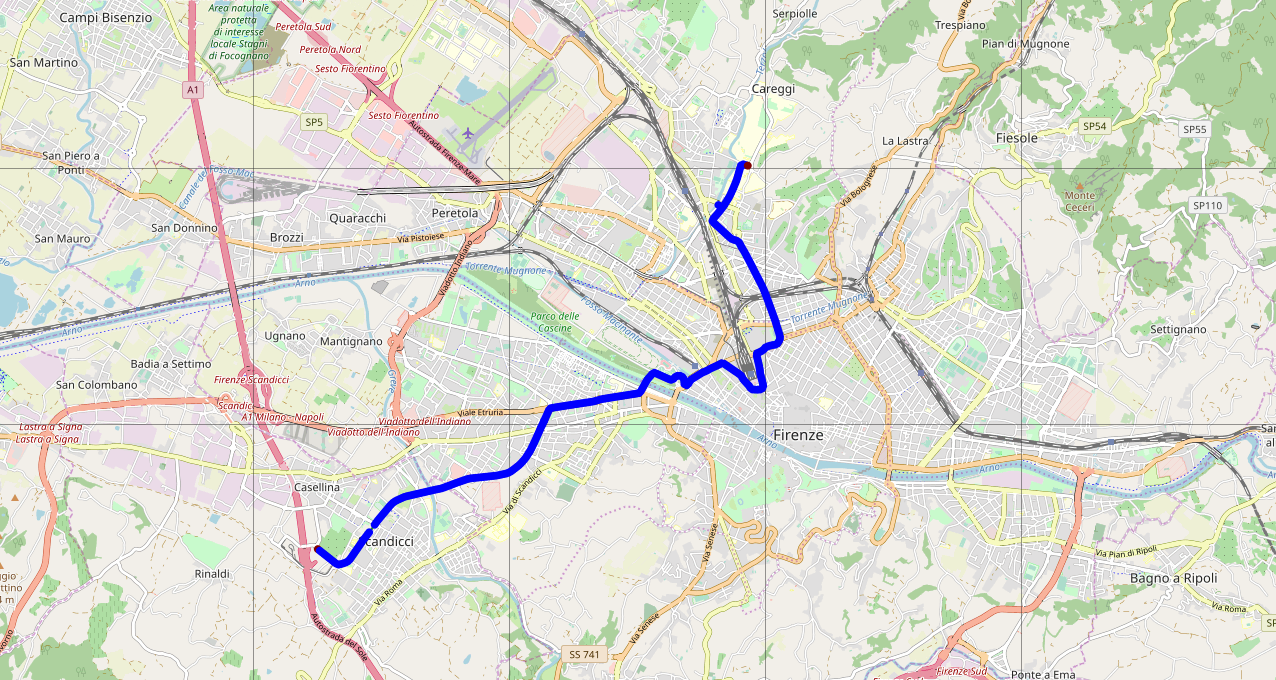
\includegraphics[width=\linewidth]{img/t1}
	\caption{Tramvia di Firenze - Linea \texttt{T1}}
	\label{fig:t1}
\end{figure}
\section{Architettura di Sistema}
Il sistema progettato ha lo scopo di eseguire SFA su una piattaforma hardware installata bordo treno, la quale riceve i dati \emph{raw} dai sensori e li elabora al fine di stimare la progressiva chilometrica del treno in ciascun istante di tempo.\\*
Tale posizione sar\`a inviata, attraverso un modem \texttt{LTE}:
\begin{itemize}
	\item All'OBCU, per essere utilizzata attivamente all'interno del sistema di \emph{interlocking}
	\item Ad un arbitario host che esegue un software grafico di tracciamento del treno: il \texttt{RailTrackTool} (RTT)
\end{itemize}
\`E possibile descrivere l'architettura di sistema a due differenti livelli: architettura a livello \emph{hardware} e architettura a livello \emph{software}.
\subsection{Architettura Hardware}
Sul treno \`e stata installata una scheda \texttt{Nvidia TX-Jetson} quale piattaforma di elaborazione dei dati. I sensori atti a campionare le misurazioni sono stati collegati alla scheda mediante appositi bus dati.\\*
Il \emph{sensor set} utilizzato in quest'applicazione \`e composto dai seguenti sensori:
\begin{itemize}
	\item \emph{Inertial Measurement Unit} (IMU):\\*
	Sensore incaricato di misurare i vettori \texttt{accelerazione} ($\mathbf{a}$) e \texttt{velocit\`a angolare} ($\mathbf{v_{ang}}$) attraverso l'uso combinato di un accelerometro e un giroscopio. Le misure di IMU sono prese rispetto a un sistema inerziale solidale con il binario e sono espresse in unit\`a stabilite dallo standard internazionale (SI):
	$$
	\mathbf{a}\;\left[\frac{m}{s^2}\right]\;\;\;\;\mathbf{v_{ang}}\;\left[ \frac{rad}{s} \right]
	$$Si tratta del sensore principale su cui si basa l'esecuzione di SFA.\newpage
	\item Odometro:\\*
	Per realizzare l'odometro \`e stato installato un rilevatore radar su una ruota del treno. Il radar misura il tempo impiegato dalla ruota a compiere un giro completo, e determina la velocit\`a angolare della ruota $\varphi'(t) = \frac{2\pi}{tempo} \left[ \frac{rad}{s}\right]$.\\*
	Noto il raggio $r\;[m]$ della ruota, \`e possibile determinare la velocit\`a lineare alla circonferenza della ruota  $x'(t)$ attraverso la relazione cinematica $x'(t) = r\varphi'(t) \left[ \frac{m\;rad}{s}\right] = r\varphi'(t) \left[ \frac{m}{s} \right]$.\\*
	Approssimando il treno come un \emph{corpo rigido}, questa sar\`a la velocit\`a lineare con cui il treno si sta muovendo.
	\item Global Positioning System (GPS):\\*
	Sensore che riceve i dati di posizione attraverso il sistema satellitare GPS.\\*
	Le misure di GPS sono riportate in formato standard come tripla di coordinate \texttt{(latitudine, longitudine, altitudine)}, rispettivamente espresse in gradi \texttt{N-S}, in gradi \texttt{E-O} e in \texttt{metri}.\\*
	In generale queste misure sono le meno affidabili in quanto la \emph{varianza} della variabile aleatoria che modella tale sorgente \`e la pi\`u significativa.
\end{itemize}
 Ad una data frequenza, i sensori inviano dati verso la scheda; quest'ultima, dopo aver eseguito un'iterazione di SFA, invia a OBCU (e/o a RTT) la stima della posizione del treno attraverso apposita modulazione di segnale elettromagnetico, in accordo con il protcollo \texttt{LTE}. Lo schema riportato in figura \ref{fig:tdiagram} mostra un diagramma dell'architettura hardware appena descritta.
\begin{figure}[h]
	\centering
	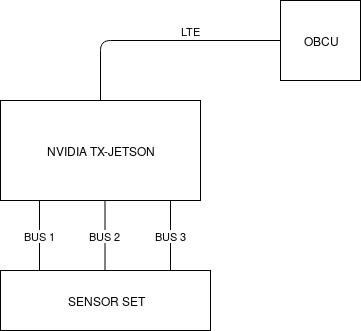
\includegraphics[width=0.7\linewidth]{img/TrainDiagram}
	\caption{Architettura hardware bordo treno}
	\label{fig:tdiagram}
\end{figure}
\subsection{Architettura Software}
Sulla scheda \`e installato il sistema operativo \texttt{Ubuntu 16.04 LTS}, basato su kernel \texttt{Linux}.\\*Qualunque software menzionato in questa Tesi \`e stato sviluppato in linguaggio \texttt{C++}.\\*
Un set di tre moduli software, denominati \texttt{interface-modules}, sono in esecuzione sulla scheda.\\*
Sia MOD\_$i$ l'$i-$esimo modulo software del set e SERIAL\_$i$ l'$i-$esima interfaccia seriale della scheda, per $i = 1,2,3$.\\*
Il funzionamento di \texttt{interface-modules} \`e il seguente:\newpage
\begin{itemize}
	\item IMU invia la coppia \texttt{(accelerazione,velocit\`a angolare)} a SERIAL\_1, MOD\_1 legge i valori da SERIAL\_1 e li invia a un secondo modulo software, denominato \texttt{listener}, attraverso l'interfaccia di rete \texttt{loopback}, in quanto \texttt{listener} esegue anch'esso sulla scheda;
	\item Odometro invia il valore di \texttt{velocit\`a lineare} a SERIAL\_2, MOD\_2 legge i valori da SERIAL\_2 e li invia a \texttt{listener};
	\item GPS invia i valori di \texttt{(latitudine, longitudine, altitudine)} a SERIAL\_3, MOD\_3 legge i valori da SERIAL\_3 e li invia a \texttt{listener}.
\end{itemize}
La comunicazione fra \texttt{interface-modules} e \texttt{listener} avviene attraverso un protocollo applicazione stabilito arbitrariamente, sia esso \texttt{INPUT\_PROTOCOL}, mentre a livello di trasporto si utilizza \texttt{UDP}.\\*
I valori ricevuti da \texttt{listener} vengono salvati in apposite \emph{strutture dati} rappresentanti misure della stessa sorgente:
\begin{itemize}
\item I vettori accelerazione e velocit\`a angolare rilevati da IMU vengono convertiti nella struttura dati \texttt{IMU\_POD};
\item La velocit\`a rilevata dal Radar/Odometro viene convertita nella struttura dati \texttt{ODO\_POD};
\item La posizione rilevata dal GPS viene infine convertita nella struttura dati \texttt{GPS\_POD}.
\end{itemize}
Il software che esegue effettivamente SFA \`e compilato come una libreria, \texttt{FusionLib}, utilizzata da \texttt{listener}. \texttt{FusionLib} dispone di interfacce software in entrata e in uscita, ossia \texttt{listener} \`e in grado di inviare le misurazioni a SFA, quali variabili di tipo \texttt{IMU\_POD, ODO\_POD, GPS\_POD} ed altres\'i di ricevere la stima della posizione del treno, essendo questo l'output dell'algoritmo, quale variabile di tipo \texttt{SFA\_OUTPUT\_POD}.\\*
Ogniqualvolta \texttt{listener} riceva un' uscita da SFA, si fa carico della comunicazione tra scheda e OBCU/RTT. Questa comunicazione, fisicamente possibile attraverso l'utilizzo del modem \texttt{LTE}, avviene utilizzando un protocollo di rete arbitrario a livello applicazione, sia esso \texttt{OUTPUT\_PROTOCOL}, mentre al livello di trasporto la scelta \`e nuovamente ricaduta su \texttt{UDP} per ragioni di efficienza.\\*
Uno schema dell'architettura software \`e quello mostrato in figura \ref{fig:tdiagramint}.\\*
\begin{figure}[h]
	\centering
	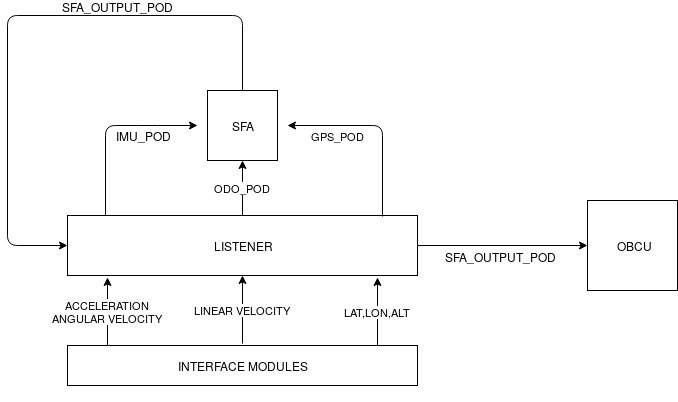
\includegraphics[width=\linewidth]{img/InternalTrainSchema}
	\caption{Architettura software bordo treno}
	\label{fig:tdiagramint}
\end{figure}\newpage
\section{Gestione della trasmissione dei dati}
Nella precedente sezione sono stati brevemente introdotti i protocolli di comunicazione implementati per gestire la comunicazione \texttt{UDP}:
\begin{itemize}
	\item Tra \texttt{interface-modules} e \texttt{listener} (\texttt{INPUT\_PROTOCOL})
	\item Tra \texttt{listener} e OBCU/RTT (\texttt{OUTPUT\_PROTOCOL})
\end{itemize}
\subsection{Trasmissione in entrata}
Per trasmettere i dati da \texttt{interface-modules} a \texttt{listener}, e dunque dai sensori al modulo software che implementa SFA, \`e stato realizzato un protocollo di comunicazione denominato \texttt{INPUT\_PROTOCOL}.\\*
Tale protocollo fa affidamento a livello trasporto su \texttt{UDP} per massimizzare la velocit\`a di trasmissione senza dover necessariamente rinunciare all'integrit\`a dei messaggi trasmessi, in quanto la comunicazione avviene tra processi in esecuzione sulla stessa macchina, e la probabilit\`a che un messaggio venga perso o che questo venga ricevuto con errori, \`e assolutamente trascurabile.\\*
Il protocollo definisce il formato del \emph{payload} del pacchetto \texttt{UDP} che contiene le informazioni di IMU, Radar/Odometro, o GPS, ed \`e descritto in tabella \ref{tab:protoin}.\\*
\begin{table}[h]
			\centering
\begin{tabular}{|c|c|c|c|}
	\hline 
	\textbf{Campo} & \textbf{Descrizione} & \textbf{Indici di bit} & \textbf{Tipo} \\ 
	\hline 
	\texttt{SENSOR\_TYPE} & ID Sensore Sorgente & 0-7 & \texttt{uint8\_t} \\ 
	\hline 
	\texttt{Seq.NO} & Numero di sequenza & 8-23 & \texttt{uint16\_t} \\ 
	\hline 
	\texttt{N\_INT} & Numero di interi trasmessi & 24-31 & \texttt{uint8\_t} \\ 
	\hline 
	\texttt{N\_DOUBLE} & Numero di double trasmessi & 31-38 & \texttt{uint8\_t} \\ 
	\hline 
\end{tabular} 
\caption{Protocollo di comunicazione in entrata}
\label{tab:protoin}
\end{table}\newpage
A discrezione del valore del campo \texttt{SENSOR\_TYPE} si distingue il tipo di informazione trasportata dal pacchetto, come descritto in tabella \ref{tab:sensors}.\\*
\begin{table}[h]
		\centering
	\begin{tabular}{|c|c|}
		\hline 
		\textbf{Valore di SENSOR\_TYPE} & \textbf{Sorgente del pacchetto} \\ 
		\hline 
		$1$ & IMU \\ 
		\hline 
		$2$ & ODOMETRO \\ 
		\hline 
		$3$ & GPS \\ 
		\hline 
		$8$ & GROUND TRUTH \\ 
		\hline 
		$9$ & STROBE \\ 
		\hline 
		$10$ & STOP \\ 
		\hline 
	\end{tabular} 
	\caption{Significato del campo SENSOR\_TYPE}
	\label{tab:sensors}
\end{table}
I pacchetti \texttt{GROUND TRUTH} sono pacchetti di inizializzazione dell'algoritmo: alla ricezione del pacchetto \texttt{GROUND TRUTH} l'algoritmo si avvia leggendo i valori trasmessi in coda al pacchetto, in accordo al valore dei campi \texttt{N\_INT} e \texttt{N\_DOUBLE}. Tali valori forniscono informazioni come progressiva chilometrica e velocit\`a iniziali del treno.\\*
I pacchetti \texttt{STROBE} sono inviati ogni secondo e forniscono un solo valore \texttt{double}, ossia un \texttt{timestamp} che l'algoritmo utilizza per sincronizzarsi.\\*
Il pacchetto \texttt{STOP} non contiene alcuna informazione utile: indica soltanto all'algoritmo di terminare l'esecuzione.\\*
Alla ricezione di un pacchetto, \texttt{listener} legge il valore del campo\\*\texttt{SENSOR\_TYPE}, e costruisce, in accordo alla relazione sorgente-struttura dati, la variabile da inviare a SFA.\\*
Il corretto ordinamento dei pacchetti trasmessi a SFA \`e garantito attraverso l'esplicito utilizzo di un buffer, codificato all'interno di \texttt{listener}, in cui i pacchetti vengono temporaneamente salvati prima di essere inviati a SFA, ed eventualmente ordinati sulla base del valore del campo \texttt{Seq.NO}.\\*
Si osservi che se l'integrit\`a non \`e minacciata dall'utilizzo di \texttt{UDP} quale protocollo di trasporto fra processi all'interno della stessa macchina fisica, altrettanto non si pu\`o dire dell'ordinamento dei messaggi. Questi potrebbero subire dei ritardi casuali in base allo stato del sistema operativo, in particolare lo \emph{scheduling} dei processi pu\`o avere influenze determinanti sullo scorretto ordinamento dei messaggi trasmessi. Utilizzando \texttt{TCP} si ovvierebbe a questa problematica, ma l'overhead insito nel protocollo stesso causerebbe un notevole degrado delle performance di SFA.
\subsection{Trasmissione in uscita}
La trasmissione dei dati in uscita da SFA avviene, in accordo al protocollo \texttt{OUTPUT\_PROTOCOL} tra \texttt{listener} e OBCU, o comunque, tra \texttt{listener} e qualunque host arbitrario che intenda ricevere le informazioni in uscita, come ad esempio un \texttt{PC} sul quale viene eseguito RTT.\\*
Come specificato, la comunicazione \`e posta in essere, a livello fisico, attraverso il protocollo \texttt{LTE}, ossia un un protocollo \emph{wireless}; mentre a livello trasporto si \`e scelto di continuare a usare \texttt{UDP} in luogo di \texttt{TCP}, col fine di massimizzare le \emph{performance} del sistema.\\*Il rischio di ricevere alcune informazioni in maniera errata, o non riceverle del tutto, \`e nettamente pi\`u elevato rispetto allo scenario precedente, nel caso in cui lo spazio fisico attraverso cui si propaga il segnale \texttt{LTE} \`e tale per cui quest'ultimo venga disturbato da sorgenti esterne.\\* Gli effetti deleteri di questa condizione sono particolarmente osservabili in alcuni tratti della linea ferrotramviaria, dove possono essere presenti numerose abitazioni e mezzi di trasporto in strada che si interpongono fisicamente tra la scheda \texttt{NVidia TX-Jetson} su cui esegue SFA e l'arbitrario host su cui viene eseguito RTT.\\*Occorre tuttavia osservare che il tracciamento del treno tramite RTT non \`e in alcun modo legato alla \emph{safety} del sistema, in quanto le funzionalit\`a \emph{safety-critical} riguardano la comunicazione tra la scheda e OBCU, ossia tra la scheda e il sistema di \emph{interlocking}.\\*
Questa problematica \`e risolta attraverso l'esplicito utilizzo di un meccanismo di \texttt{acknowledgment} simile a quello utilizzato da \texttt{TCP}: ciascun pacchetto in uscita da SFA viene indicizzato con un \emph{sequence number} e, in ricezione, viene inviato ogni secondo un \emph{ack} replicante l'ultimo numero di sequenza correttamente ricevuto. Solo quando il mittente riceve l'ack $i$ dal destinatario invier\`a il messaggio contenente l'uscita indicizzata con \emph{sequence number} $i+1$.\\*
Anche in questo caso, il protocollo definisce il formato del \emph{payload} del pacchetto \texttt{UDP} inviato da \texttt{listener}, ed \`e riportato in tabella \ref{tab:protoout}.\\*\newpage
\begin{table}[h]
	\centering
	\begin{tabular}{|c|c|c|c|}
		\hline 
		\textbf{Campo} & \textbf{Descrizione} & \textbf{Indici di bit} & \textbf{Tipo} \\ 
		\hline
		\texttt{Seq.NO} & Numero di sequenza & 0-15 & \texttt{uint16\_t} \\ 
		\hline 
		\texttt{ECEF\_X} & Coordinata X del treno & 16-79 & \texttt{double} \\ 
		\hline 
		\texttt{ECEF\_Y} & Coordinata Y del treno & 80-143 & \texttt{double} \\ 
		\hline 
		\texttt{ECEF\_Z} & Coordinata Z del treno & 144-207 & \texttt{double} \\ 
		\hline 
		\texttt{FU\_ARC\_LEN} & Progressiva chilometrica & 208-271 & \texttt{double} \\ 
		\hline 
	\end{tabular} 
\caption{Protocollo di comunicazione in uscita}
\label{tab:protoout}
\end{table}
In ricezione dovr\`a essere inviato il pacchetto \emph{ack} al mittente, ed il suo formato \`e descritto in tabella \ref{tab:ack}.
\begin{table}[h]
	\centering
	\begin{tabular}{|c|c|c|c|}
	\hline 
	\textbf{Campo} & \textbf{Descrizione} & \textbf{Indici di bit} & \textbf{Tipo} \\ 
	\hline
	\texttt{ACK} & Ultimo \texttt{Seq.NO} & 0-15 & \texttt{uint16\_t} \\ 
	\hline
\end{tabular}
\caption{Formato del pacchetto di \emph{ack}}
\label{tab:ack}
\end{table}
Si osserva che SFA produce la stima della posizione del treno sia in termini di progressiva chilometrica che di coordinate \texttt{ECEF}.\\*
\texttt{ECEF} \`e acronimo di \emph{Earth Centered Earth Fixed} ed \`e uno standard che misura le coordinate geografiche di un oggetto come la terna $ P = (x,y,z)$. Ciascuna coordinata viene espressa considerando la \emph{proiezione su piano} della Terra, e prendendo come origine $O$ l'intersezione fra l'equatore e il meridiano di \emph{Greenwich}.\\*
Le coordinate \texttt{ECEF} misurano tre lunghezze, pertanto in accordo a SI, esse sono espresse in \texttt{metri}.
